\chapter{Riconoscitori con PDA}

Un RSF \underline{non può riconoscere} un linguaggio di tipo 2, ha un limite intrinseco alla capacità di memorizzazione: non riesce a riconoscere frasi che richiedano di memorizzare una parte di lunghezza non nota a priori.

\textbf{Esempio}: bilanciamento delle parentesi $L = {(^n c )^n, n \ge 0}$, $G = {S \rightarrow (S)\ |\ c}$

In questo linguaggio il prefisso $(^n$ non ha lunghezza limitabile a priori.

\section{Push-Down Automaton (PDA)}
Un PDA è un RSF con aggiunto uno stack, con stack non ci si riferisce a una struttura dati fisica ma a un suo modello astratto, ovvero una sequenza di simboli, definito in modo tale che si possa operare soltanto su quello in "cima".

Il PDA legge un simbolo d'ingresso e transita in un nuovo stato, in più a ogni passo altera lo stack, producendo una nuova configurazione.

Un PDA può prevedere $\varepsilon$-mosse, ovvero transizioni spontanee che manipolano lo stack senza consumare simboli in ingresso.

Un PDA è una sestupla:

{\centering
$\langle A,\ S,\ S_0,\ sfn,\ Z,\ Z_0\rangle$\par}
dove:
\setlist{nosep}
\begin{itemize}
    \item $A$ = alfabeto
    \item $S$ = insieme degli stati
    \item $S_0$ = stato iniziale $\in S$
    \item $sfn: (A\cup \varepsilon) \times S \times Z \rightarrow W$
    \item $Z$ = alfabeto dei \underline{simboli interni} 
    \item $Z_0 \in Z$ = simbolo iniziale sullo stack
\end{itemize}
\setlist{}

\begin{figure}[H]
    \caption{Struttura PDA}
    \centering
    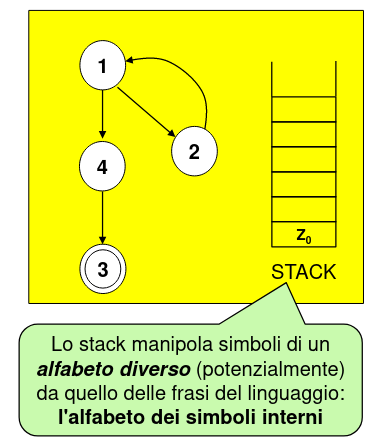
\includegraphics[width=0.4\textwidth]{/home/riccardoob/appunti/linguaggi/images/13.png}
\end{figure}

Il linguaggio \underline{accettatto} da un PDA è definibile in 2 modi equivalenti:
\begin{itemize}
    \item \textbf{Criterio dello stato finale}: il linguaggio accettato è l'insieme di tutte le stringhe di ingtesso che portano il PDA in uno degli stati finali.
    \item \textbf{Criterio dello stack vuoto}: il linguaggio accettato è definito come l'insieme di tutte le stringhe di ingresso che portano il PDA nella configurazione di \textit{stack vuoto}.
\end{itemize}

La funzione sfn, dati:
\begin{itemize}
    \item un \textit{simbolo in ingresso} $a\in A$
    \item lo \textit{stato attuale} $s\in S$
    \item il simbolo interno attualmente al \textit{top dello stack} $z\in Z$
\end{itemize}
opera come segue:
\begin{itemize}
    \item \textbf{consuma} il simbolo di ingresso $a$
    \item effettua il \textbf{POP} dello dallo stack, prelevando il simbolo $z$
    \item porta l'automa in stato futuro $s' = sfn(a, s, z)_{\prod S}$
    \item effettua una \textbf{PUSH} sullo stack di zero o più simboli interni $z'\in Z$\\ $z' = sfn(a, s, z)_{\prod S}$
\end{itemize}

Si consideri il linguaggio generato da:
\begin{itemize}
    \item $A = \{0, 1, c\}$
    \item $P = \{S \rightarrow 0\ S\ 0\ |\ 1\ S\ 1\ |\ c\}$
    \item $L = \{\texttt{word}\  c\ \texttt{word}^R\}$
\end{itemize}

Definiamo il PDA come segue:
\begin{itemize}
    \item $A = \{0, 1, c\}$
    \item $S = \{Q1=S_0, Q2\}$
    \item $Z = \{Zero, Uno, Centro\}$
\end{itemize}

\begin{figure}[H]
    \centering
    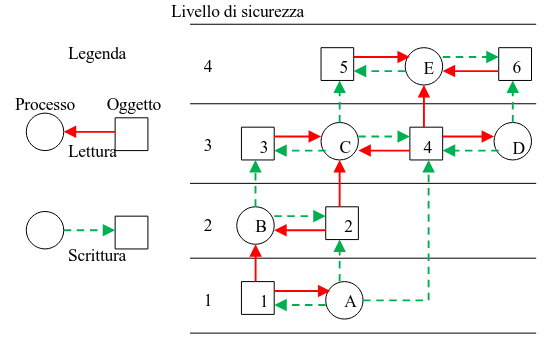
\includegraphics[width=0.5\textwidth]{/home/riccardoob/appunti/linguaggi/images/14.png}
\end{figure}

\subsection{PDA non deterministici}
Anche un PDA può essere non deterministico: in tal caso, la funzione $sfn$ produce insiemi di elementi $W$ ($W$ sottoinsieme finito di $S \times Z^*$).

Ad esempio, il PDA tale che $sfn(Q_0, a, Z) = \{(Q_1, Z_1)(\cdots)(Q_k, Z_k)\}$ è \textbf{non deterministico} in quanto l'automa, nello stato $Q_0$, con simbolo interno in cima allo stack $Z$ e ingresso $a$ ha \underline{più di uno stato futuro possibile} in base alla evoluzione cambia anche il se di simboli da porre nello stack.

\noindent
\textbf{TEOREMA}\\
La classe dei linguaggi riconosciuti da un PDA non-determistico coincide con la classe dei linguaggi context-free: perciò qualunque linguaggio context-free può sempre essere riconosciuto da un opportuno PDA.

É possibile rinunciare al determinismo?\\
In generale no:

\noindent
\textbf{TEOREMA}\\
Esistono linguaggi context-free riconoscibili soltanto da PDA non-deterministici.

ma in molti casi di interesse pratico esistono linguaggi context-free riconoscibili da PDA deterministici: \underline{linguaggi context-free deterministici}. 


\subsection{PDA deterministici}
Cosa serve per ottenerlo?

Viste le condizioni precedenti, non deve succedere che l'automa, in dato stato $Q_0$, con simbolo in cima allo stack $Z$ e ingresso $x$ possa:
\begin{itemize}
    \item portarsi in \underline{più stati futuri} 
        $sfn(Q_i, x, Z) = \{(Q_1, Z_1), (\cdots), (Q_k, Z_k)\}$
    \item optare se leggere o non leggere il simbolo di ingresso $x$ a causa della presenza di entrambe le mosse $sfn(Q_i, x, Z)$ e $sfn(Q_i, \varepsilon, Z)$
\end{itemize}

\underline{Unendo}, \underline{intersecando} o \underline{concatenando} linguaggi deterministici,  non necessariamente si ottiene un linguaggio deterministico.

I \underline{complemento} di un linguaggio è deterministico.

Con $L$ linguaggio deterministico e $R$ linguaggio regolare, il \underline{linguaggio quoziente}  $L/R$ (insieme di stringhe di $L$ private di suffisso regolare) è deterministico.

Con $L$ linguaggio deterministico e $R$ linguaggio regolare, il \underline{concatenamento} $L.R$ (insieme di stringhe di $L$ cun suffisso regolare) è deterministico.

\subsubsection{Sottoclassi particolari}
Per un PDS \textbf{deterministico}:
\begin{itemize}
    \item il criterio dello \underline{stack vuoto} risulta meno potente del criterio \underline{stati finali}
    \item una limitazione sul numero di stati intenro o sul numero di configurazioni finali riduce l'insieme dei linguaggi riconoscibili
    \item l'assenza di $\varepsilon$-mosse riduce l'insieme dei linguaggi riconoscibili
\end{itemize}


\subsection{Realizzazione di PDA deterministici}
Possibilità di seguire la definzione, ma non molto pratico.

Si adotta un approccio che manipoli uno stack con la stessa logica di un PDA, dove lo stack è la vera differenza, ad esempio una macchina virtuale che abbia uno stack può essere fatta funzionare come PDA, opportunamente pilotata.

Si potrebbe controllare "a mano" lo stack, oppure in modo automatico attraverso le \underline{chiamate ricorsive di funzioni}, dove sono già gestiti stack relativi alla ricorsione.

\subsubsection{Top-Down Recursive-Descent Parsing}

Con l'\textbf{analisi ricorsiva discendente} si introduce \underline{una funzione per ogni metasimbolo} della grammatica, e la si chiama ogni volta che si icontra quel metasimbolo.

Ogni funzione copre le regole di quel metasimbolo, ossia riconosce il sotto-linguaggio corrispondente:
\begin{itemize}
    \item termina normalmente (o segno di successo) se incontra simboli coerenti
    \item abortisce (o restituisce un segno di fallimento) se incontra simboli non coerenti
\end{itemize}

\subsubsection{Esempio}

Il solito linguaggio $L = \{\texttt{word}\ c\ \texttt{word}^n\}$, alfabeto $A = \{0,\ 1,\ c\}$ e regole $S \rightarrow 0\ S\ 0\ |\ 1\ S\ 1\ |\ c$. 

\begin{itemize}
    \item Introdurre tante funzioni quanti i metasimboli, qui una sola $S()$.
    \item Chiamare una funzione ogni volta che si incontra il suo metasimbolo
    \item Ogni funzione deve coprire le regole di quel metasimbolo
        \begin{itemize}
            \item se il simbolo d'ingresso è 0 $\rightarrow$ seguire la prima regola
            \item se il simbolo d'ingresso è 1 $\rightarrow$ seguire la seconda regola
            \item se il simbolo d'ingresso è c $\rightarrow$ seguire la terza regola
        \end{itemize}
\end{itemize}

Nel caso della prima regola, consumiamo il carattere di ingresso 0, invochiamo la funzione $S()$ e consumiamo un nuovo carattere d'ingresso e verifichiamo che sia 0.

Se la verifica ha esito positivo, significa che la funzone ha incontrato simboli coerenti con le proprie regole.

Se la verifica ha esito negativo, significa che la funzione ha incontrato simboli che non corrispondono alle sue regole.

\underline{\textbf{finisci slide esempio 24-28!!!!!!!!!!!!!!!!!!!!!!!!!!!!!!!!!!!!!!!!!!!!!!!!!!!!!!!!!!!!!!!!!!!!!!!!!!!!}}

\subsection{Separare motore e grammatica}
Applicare l'analisi ricorsiva discendente è un processo meccanico, che tuttavia introduce informazioni cablate nel codice, difficili da aggiornare.

É possibile separare il \textbf{motore}, invariante rispetto alle regole, dalle \underline{regole della grammatica}; si presta a questo scopo la \underline{tabella di parsing}, simile alla tabella delle transizioni di un RSF, indica però la prossima \textit{produzione} da applicare.

Il motore prenderà singole decisioni consultando questa tabella.

\subsubsection{Parsing tables - esempi deterministici}

\paragraph{Linguaggio} $L = \{\texttt{word}\ c\ \texttt{word}^n\}$

\begin{figure}[H]
    \centering
    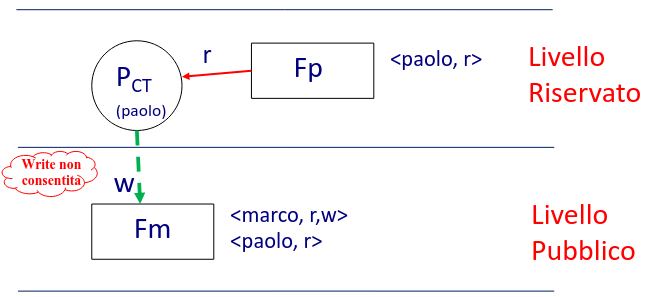
\includegraphics[width=0.8\textwidth]{/home/riccardoob/appunti/linguaggi/images/15.png}
\end{figure}

\paragraph{Linguaggio} $L = \{\texttt{if}\ \texttt{c}\ \texttt{then}\ \texttt{cmd}\ (\ \texttt{endif}\ |\ \texttt{else}\ \texttt{cmd}\ )\ \}$ 

\paragraph{Produzioni} $S \rightarrow \texttt{if}\ \texttt{c}\ \texttt{then} \ \texttt{cmd} \ \texttt{X} $, $\texttt{X}  \rightarrow \texttt{endif}\ |\ \texttt{else}\ \texttt{cmd} $ 

\begin{figure}[H]
    \centering
    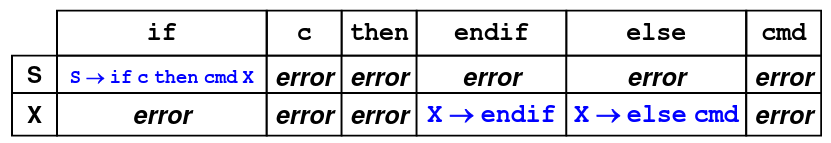
\includegraphics[width=0.8\textwidth]{/home/riccardoob/appunti/linguaggi/images/16.png}
\end{figure}

\subsection{Analisi ricorsiva discendente - vantaggi e limiti}
Vantaggi
\begin{itemize}
    \item immediata scrittura del riconoscitore
    \item migliore leggibilità a modificabilità del codice
    \item facilitata inserzione di azioni nella fase di analisi
\end{itemize}
Svantaggi
\begin{itemize}
    \item non sempre applicabile
    \item funzionale solo se non esistono ambiguità sulla regola da applicare
\end{itemize}

Si individua una sottoclasse di grammatiche context-free che garantisce il determinismo dell'analisi sintattica.

Per rendere deterministica l'analisi ricorsiva, si rende necessario avere una visione del \textit{passato} dell'analisi (simboli consumati fino a quel punto) e una del \textit{futuro}, generalmente un solo carattere in avanti.

\section{Grammatiche $LL(k)$}
Si definiscono \textit{grammatica $LL(k)$} quelle che sono analizzabili in modo deterministico:
\begin{itemize}
    \item procedendo \textit{left to right}
    \item applicando \textit{left-most derivation}
    \item guardando avanti al più \textit{k} simboli
\end{itemize}

Ricoprono un posto fondamentale le grammatiche LL(1), ovvero quelle in cui basta guardare un simbolo in avanti per operare in modo deterministico.

\subsubsection{Esempio}
Si consideri la grammatica
\begin{itemize}
    \item $\texttt{VT}\ =\ \{\texttt{p},\ \texttt{q},\ \texttt{a},\ \texttt{b},\ \texttt{d},\ \texttt{x},\ \texttt{y}\}$
    \item $\texttt{VN}\ =\ \{\texttt{S},\ \texttt{X},\ \texttt{Y}\}$
\end{itemize}

Produzioni
\begin{equation*}
    \begin{aligned}
        &\texttt{S} \rightarrow \texttt{p}\ \texttt{X}\ &&|\ \texttt{q}\ \texttt{Y}\\
        &\texttt{X} \rightarrow \texttt{a}\ \texttt{X}\ \texttt{b}\ &&|\ \texttt{x}\\
        &\texttt{Y} \rightarrow \texttt{a}\ \texttt{Y}\ \texttt{d}\ &&|\ \texttt{y}
    \end{aligned}
\end{equation*}

Le parti \textbf{destre} delle produzioni di uno stesso meta simbolo, iniziano tutte con un simbolo terminale diverso, è sufficiente guardare avanti di un carattere per scegliere con certezza la produzione per scegliere con certezza la produzione con cui proseguire l'analisi.

Creando la parsing table, si nota che ogni cella contiene una sola produzione, quindi non si hanno ambiguità sulle prossime mosse da fare, è facile vedere che il parser è deterinistico.

\begin{figure}[H]
    \centering
    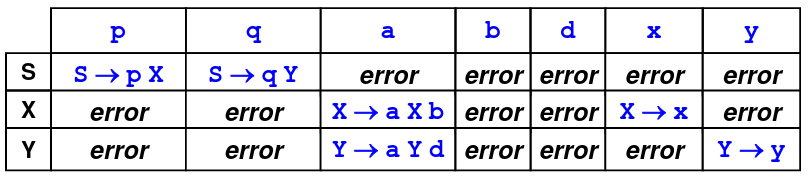
\includegraphics[width=0.8\textwidth]{/home/riccardoob/appunti/linguaggi/images/17.png}
\end{figure}

La frase di inzio deve essere completa oppure può essere parziale? Nel caso in cui si voglia imporre che la frase deve essere finale occorre imporre una regola \textit{top-level} che specifica che la frase deve terminare con \texttt{\$}, carattere che rappresenta il fine stringa/linea/file del tipo $\texttt{Z} \rightarrow \texttt{S}\ \$$ .

\subsection{Starter Symbol Set}
Spesso le parti destre delle produzioni di uno stesso metasimbolo non iniziano tutte con un simbolo terminale, non è chiaro quali siano gli input ammissibili.

Occorre ridefinire il concetto di simbolo iniziale $\rightarrow$ \underline{Starter Symbols Set}.

Lo starter symbols set della riscrittura $\alpha$ è l'insieme
\begin{equation*}
    SS(\alpha) = \{ a \in \texttt{VT}\ |\ \alpha \xrightarrow{}\mathrel{\vphantom{\to}^*} a\ \beta\}, \texttt{ con } \alpha \in V^+ \texttt{ e } \beta \in V^*
\end{equation*}

In sostanza gli starter symbols sono le iniziali di una forma di frase $\alpha$, ricavate applicando con più produzioni.
L'operatore $*$ cattura il caso limite in cui $\alpha \in VT$, ossia già terminale, e non richiede di applicare derivazioni.

Per includere anche il caso $\alpha \rightarrow \varepsilon$, si introduce l'insieme
\begin{equation*}
\texttt{FIRST}(\alpha ) = \texttt{trunc}_1(\{x \in VT^*\ |\ \xrightarrow{}\mathrel{\vphantom{\to}^*}\}), \texttt{ con } \alpha \in V^*
\end{equation*}

dove $\texttt{trunc}_1$ denota il troncamento della stringa al primo elemento.

Generalizzando la regola precendete, condizione necessaria perché una grammatica sia $LL(1)$ è che gli \textit{start symbols} relativi alle parti destre di uno stesso metasimbolo siano disgiunti.

\textbf{\underline{Esempi 44-52???????????????????????????????????????????????????????????????????????????????????????????}} 

É possibile capire in modo più rapido se una grammatica è $LL(1)$?

Due opzioni:
\begin{itemize}
    \item agire sulla parsing table, formalizzando il concetto di \textbf{blocco annullabile} e integrando nella tabella l'informazione sulle stringhe che possono scomparire.
    \item ampliare la nozione di starte symbols set con i \underline{Director Symbols} set (o \underline{Look-Ahed} set)
\end{itemize}

\underline{\textbf{inserisci slide 55-67!!!!!!!!!!!!!!!!!!!!!!!!!!!!!!!!!!!!!!!!!!!!!!!!!!!!!!!!!!!!!!!!!!!!!!!!!!!!!!!!!!!!!!!!!!!!!!!1}}  













